\subsection{Backtracking}

El backtracking és un algorisme que resol els problemes de forma recursiva considerant totes les combinacions possibles per resoldre un problema i que construeix la solució de manera ascendent, una peça a cada torn, també descarta totes aquelles solucions que no satisfan les limitacions del problema en qualsevol moment.

S'utilitza el backtracking en els següents problemes:

\begin{itemize}
    \item Problema de decisió -> Es busca una solució factible.
    \item Problema d'optimització -> Es busca una solució òptima
    \item Problema d'enumeració -> Es busquen totes les solucions factibles.
\end{itemize}

Tot i això, la majoria de problemes que es resolen amb backtracking també es poden resoldre amb altres algorismes com greedy o programació dinàmica amb una complexitat temporal $O(log n)$, $O(n)$, $O(n log n)$.

No obstant això, hi ha problemes que encara només poden ser resolts amb backtracking.
\newline

Un problema típic que es pot resoldre amb backtracking és el conegut problema de les N reines.
Aquest problema consisteix a trobar una distribució de $n$ reines en un tauler de $n * n$ de mode tal que les reines co\lgem ocades en el tauler no s'ataquin entre elles. Així, dues reines no es poden trobar en la mateixa fila, columna o diagonal.

Aquest problema té dues versions. La més simple consisteix a buscar una solució vàlida per una $n$ donada. L'altra versió, més difícil, consisteix a contar el nombre de solucions possibles per una $n$ donada, és a dir s'ha de comptar totes les diferents maneres de co\lgem ocar les reines de forma vàlida.

El problema te l'has d'imaginar com un arbre en el qual cada branca és un camí que pots triar, és a dir, una posició de la reina en el taulell, llavors després l'algorisme comprova si aquella posició és vàlida (la reina no s'ataca amb totes les altres reines), si no és vàlida la posició, descartes la branca i passes a la següent, en cas contrari segueixes amb la branca fins que aquesta és descartada o fins que arribes a co\lgem ocar les $n$ reines i, per tant, ja has trobat una solució possible, si volguessis fer la segona versió del problema, llavors hauries de continuar mirant les altres branques per comprovar si poden portar a altres solucions diferents i així fins que s'acaben totes les branques, en aquest cas el programa ha de parar i et retorna el nombre de solucions que ha trobat.

En el següent codi podem observar la major part de la implementació de la versió fàcil del problema de les N reines (cal recalcar que si n = 2 o n = 3, no existeix cap distribució de reines vàlida).
\newpage


\begin{lstlisting}
bool esSegur(int fil, int col){
    int i, j;
    // mirem si algunes reines s'ataquen entre elles
    for (i = 0; i < col; i++)
        if (Tauler[fil][i])
            return false;
 
    for (i = fil, j = col; i >= 0 && j >= 0; i--, j--)
        if (Tauler[i][j])
            return false;
 
    for (i = fil, j = col; j >= 0 && i < n; i++, j--)
        if (Tauler[i][j])
            return false;
 
    return true;
}

bool backtracking(int col){  // Input -> 5 (reines)
    if (col == n){ // hem colocat les n reines
        printSol();
        return true;  
    }      

    for (int i = 0; i < n; i++){
        if (esSegur(i, col)){
            Tauler[i][col] = 1; // la posició és vàlida (reina) 
            if (backtracking(col + 1))
                return true;
            
            Tauler[i][col] = 0; // provem una altra possibilitat
        }
    }   
    return false;
}

void printSol(){
    for (int x = 0; x < n; x++){
        for (int y = 0; y < n; y++)
            cout << Tauler[x][y] << " ";
        cout << endl;
    }
    // Output -> 1 0 0 0 0 
    //            0 0 0 1 0 
    //            0 1 0 0 0 
    //            0 0 0 0 1 
    //            0 0 1 0 0 
}
\end{lstlisting}



\begin{center}
    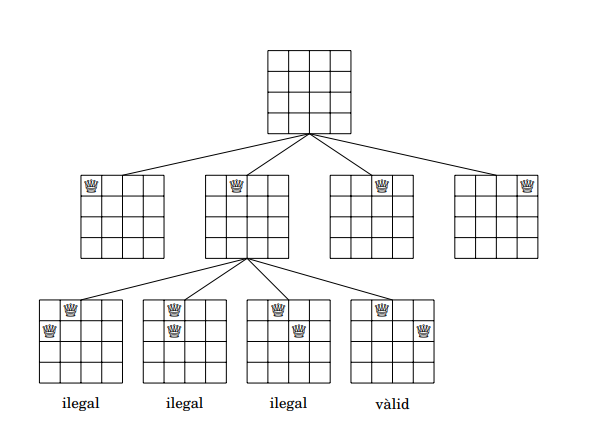
\includegraphics[width=.8 \textwidth]{back.png}
    
    \caption{\emph{Figura 5: Petita part de l'arbre de possibilitats que genera el backtracking amb $n = 4$. Font: \url{https://cses.fi/book/book.pdf}}}
\end{center}



Un altre exemple de l'ús del backtracking és quan es vol imprimir tots els subconjunts que es poden formar a partir d’un conjunt de paraules.

Plantegem el problema com un llistat de booleans i per cada paraula hem de decidir amb veritat o fals si agafem la paraula o no, per fer-ho més entenedor ens ho hem d'imaginar de nou com un arbre en el qual si vas per la branca de l'esquerra, vol dir que no agafes la paraula en canvi si vas cap a la dreta, sí que l'agafes, finalment quan arribem al final d'una branca, imprimim el subconjunt.


\begin{center}
    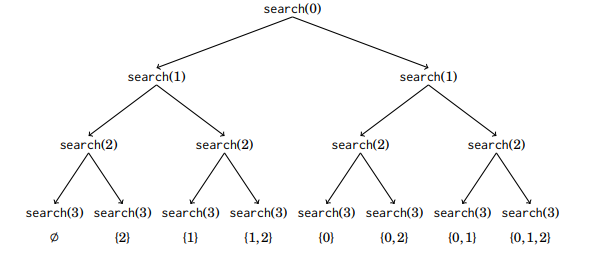
\includegraphics[width=.9 \textwidth]{back2.png}
    \caption{\emph{Figura 6: Arbre de decisions que es formaria amb un conjunt de números [0,1,2]. Font: \url{https://cses.fi/book/book.pdf}}}
\end{center}

\newpage

En el següent codi, observem la implementació de l'exemple mencionat anteriorment. \newline


\begin{lstlisting}
vector<string> paraules;

void backtracking(int i, vector<bool> bools){
    if (i == n) {   // cas base de la recursió
        cout << "{";
        for (int i = 0; i < n; i++)
            if (bools[i] == true)
                cout << paraules[i] << ", ";
        cout << "}" << endl;
        return;
    }
    bools[i] = 0;  // fem backtracking
    backtracking(i + 1, bools);  // cas recursiu
    bools[i] = 1;  // fem backtracking
    backtracking(i + 1, bools);  // cas recursiu
}

// Si el conjunt de paraules fos ["hola", "hi", "bonjour"]

// L'output seria el següent:
//  {}
//  {bonjour}
//  {hi}
//  {hi, bonjour}
//  {hola}
//  {hola, bonjour}
//  {hola, hi}
//  {hola, hi, bonjour}

// Observem que concorda amb la imatge anterior.
\end{lstlisting}






